Pasek, umieszczony po lewej stronie ekranu nosi nazwę Launchera (ang: \textcolor{ubuntu_orange}{Wyzwalacz}). Launcher umożliwia przechowywanie skrótów do ulubionych i najczęściej użytkowanych aplikacji, dostęp do uruchomionych programów, zamontowanych urządzeń (pamięć USB/SD, zewnętrzne dyski twarde, CD/DVD) oraz kosza. Uruchomiona aplikacja w systemie, na czas swojej pracy, umieszcza w obrębie Launchera swoją ikonę.

\subsubsection{Uruchamienie programów z Launchera}
\begin{wrapfigure}{l}{0.1\textwidth}
	\vspace{-10pt}
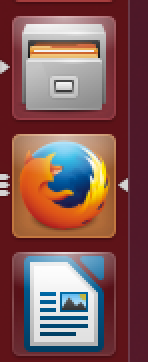
\includegraphics[width=\linewidth]{images/unity_launcher_programy.png}
\end{wrapfigure}

Aby uruchomić program bezpośrednio z Launchera wystarczy pojedyncze kliknięcie lewym przyciskiem myszy na ikonie wybranego programu. Uruchomione programy mają podświetlone ikony oraz niewielki trójkącik po swojej lewej stronie. Aby uruchomić kolejną kopię programu kliknij lewym przyciskiem myszy na jego ikonę trzymając wciśnięty klawisz \keys{Shift}.

\noindent Liczba trójkątów po lewej stronie programu oznacza ilość otwartych kopi danego programu. Jak łatwo się domyślić, gdy ikona nie posiada żadnego trójkącika, to program jest wyłączony. Program, który aktualnie używamy (aktywne okno) jest oznaczone niewielkim trójkącimkiem po prawej stronie ikony.

\noindent Na rysunku obok może zobaczyć ikonę programu Pliki (menadżer plików Nautilus), który jest uruchomiony jeden raz. Tło ikony jest podświetlone.\\
Ikona przeglądarki Internetowej Firefox ma trzy trójkąty po lewej. Oznacza to, że została uruchomiona w trzech osobnych instancjach. Jedna z kopi Firefoksa jest akurat w użyciu, co sygnalizuje trójkącik po prawej. Tło ikony jest podświetlone.\\
Trzecia ikona na rynku (Skrót do procesora tekstu LibreOffice Writer) jest nieaktywna. Ten program nie jest aktualnie uruchomiony.

\subsubsection{Zarządzanie otwartymi oknami}
Kliknięcie lewym przyciskiem myszy na ikonę uruchomionego programu przenosi do otwartego okna. Jeżeli dany program ma więcej niż jedną instancję to pokazane zostaną miniatury wszystkich okien aplikacji. Klikając lewym przyciskiem myszy możesz wybrać, o które okna ci chodzi. 

Kółkiem myszy możesz się pomiędzy instancjami programu. Umieść kursor myszy nad ikoną aplikacji i poruszaj kółkiem myszy w górę lub w dół aby przejść do następnej/poprzedniej instancji programu.

\subsubsection{Zmiana położenia ikon}
\begin{wrapfigure}[5]{l}{0.25\textwidth}
	\vspace{-10pt}
	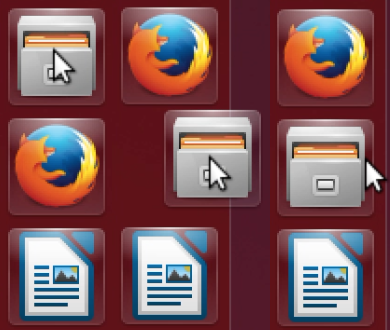
\includegraphics[width=\linewidth]{images/unity_launcher_zmiana_polozenia_ikon.png}
\end{wrapfigure}

Zawartość Launchera, poza ikoną Dasha oraz kosza, może być dowolnie modyfikowana. Aby zmienić położenie ikony na panelu, umieść kursor myszy w obrębie ikony, wciśnij i przytrzymaj lewy przycisk myszy. Kiedy ikona zostanie odczepiona od Launchera przesuń ją na wybrane przez siebie miejsce i puść przycisk myszy.

\subsubsection{Dodawanie ikon do Launchera}
Skrót do programu na Launcherze można dodać na dwa sposoby i należy do tego wykorzystać okno Dasha (o którym będzie później). Aby dodać ikonę na pasek bezpośrednio z okna Dasha, należy odszukać program i przeciągnąć jego ikonę w dowolne miejsce na pasek Launchera.

Druga metoda polega na uruchomieniu programu. Następnie należy nacisnąć prawym przyciskiem myszy na ikonie uruchomionego programu i z widocznego menu kontekstowego wybrać \textcolor{ubuntu_orange}{Dodaj do panelu uruchamiania}.

\subsubsection{Usuwanie ikon z Launchera}
Ikonę z panelu można usunąć na dwa sposoby. Chwyć ikonę kursorem myszy i przenieść ją do kosza lub po naciśnięciu prawym przyciskiem myszy na ikonie, z wyświetlonego menu kontekstowego wybierz \textcolor{ubuntu_orange}{Usuń z panelu uruchamiania}.

\subsubsection{Szybka Lista menu kontekstowego (QuickList)}
\begin{center}
	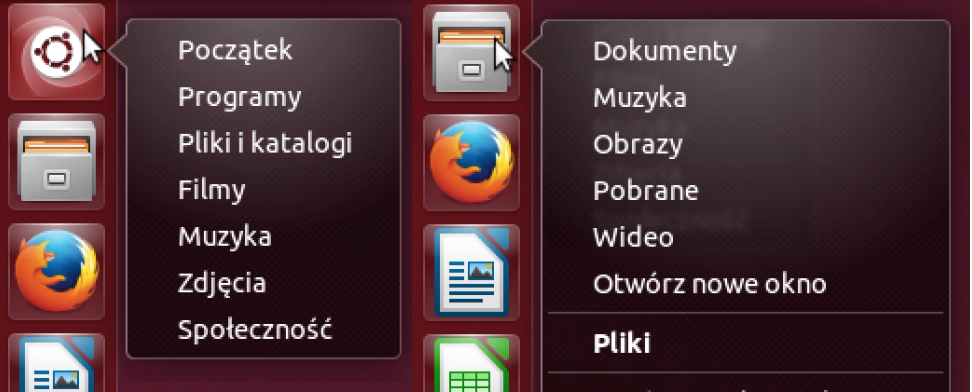
\includegraphics[width=\linewidth]{images/unity_launcher_quicklist.png}
\end{center}

Jedną z ciekawszych funkcjonalności Launchera jest QuickList (SzybkaLista). Programy umieszczone na Launcherze mogą w swoim menu kontekstowym umieszczać różne polecenia. Na powyższej grafice widać dwa przykłady. Po lewej mamy menu kontekstowe Dasha, zawierające skróty do zainstalowanych soczewek (zostanie to omówione w kolejnym rozdziale). Po prawej widać menu kontekstowe menadżera plików, zawierające skróty do najważniejszych katalogów użytkownika. Przeglądarka internetowa Firefox pozwoli dodatkowo uruchomić okna anonimowego przeglądania.
\clearpage